\documentclass[a4paper, 10pt, final, garamond]{book}
\usepackage{cours-preambule}

\makeatletter
\renewcommand{\@chapapp}{Chimie -- chapitre}
\renewcommand\thechapter{4 et 5}
\makeatother
\renewcommand{\theequation}{5.\arabic{equation}}
\renewcommand{\thefigure}{\arabic{figure}}

\hfuzz=5.002pt

% \toggletrue{student}
% \toggletrue{corrige}
% \renewcommand{\mycol}{black}
\renewcommand{\mycol}{gray}

\begin{document}
\setcounter{chapter}{7}

\settype{enon}
\settype{solu_prof}
\settype{solu_stud}

\chapter{\cswitch{Correction du TD}{TD~: Acide-base et précipitation}}

\resetQ
\section{Acide carbonique}
\enonce{%
	On considère l'acide carbonique, un diacide ($\pk[1] = \num{6.4}$ et $\pk[2] =
		\num{10.3}$) dans l'eau.
}
\QR{%
	Écrire les équilibres liant les espèces des couples \ce{H2CO3}/\ce{HCO3-} et
	\ce{HCO3-}/\ce{CO3^2-}
}{%
	\begin{alignat}{3}
		\beforetext{$K_{A,1}$}
		\ce{H_2CO3\aqu{}  & + H_2O\liq{} & = & HCO_3^-\aqu{} & + H_3O^+\aqu{}}
		\tag{1}
		\\
		\beforetext{$K_{A,2}$}
		\ce{HCO_3^-\aqu{} & + H_2O\liq{} & = & CO_3^2-\aqu{} & + H_3O^+\aqu{}}
		\tag{2}
	\end{alignat}
}
\QR{%
	Exprimer les constantes d'acidité associées aux deux couples en fonction de
	concentrations à l'équilibre.
}{%
	\[
		K_1 = \frac{[\ce{H_3O+}]\ind{eq}[\ce{HCO_3^-}]\ind{eq}}
		{[\ce{H_2CO_3}]\ind{eq}c^\circ}
		\qqet
		K_1 = \frac{[\ce{H_3O+}]\ind{eq}[\ce{CO_3^2-}]\ind{eq}}
		{[\ce{HCO_3^-}]\ind{eq}c^\circ}
	\]
}
\QR{%
	Préciser sur un axe gradué en pH les domaines de prédominance des différentes
	espèces.
}{%
	\begin{center}
		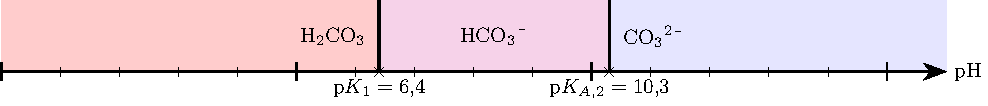
\includegraphics[width=\linewidth]{predom_ex1}
	\end{center}
}
\QR{%
	Écrire la réaction entre \ce{H2CO3} et \ce{CO3^2-}. Quelle est la valeur de la
	constante d'équilibre~?
}{%
	\begin{gather*}
		\beforetext{$K_3$}
		\ce{H_2CO_3\aqu{} + CO_3^2-\aqu{} = 2HCO_3^-\aqu{}}
		\tag*{$(3) = (1)-(2)$}
		\\\Ra
		\boxed{K_3 = \frac{K_{A,1}}{K_{A,2}}}
		\Lra
		\xul{K_3 = 10^{\num{3.9}}}
	\end{gather*}
}
\QR{
	Déterminer l'espèce majoritaire dans les trois solutions $S_1, S_2$ et $S_3$
	caractérisées par~:
  \begin{tasks}(3)
    \task 
		$\pH_{S_1} = \num{3}$
    \task 
		$[\ce{H_3O+}]_{S_2} = \SI{1e-8}{mol.L^{-1}}$
    \task 
  $[\ce{HO-}]_{S_3} = \SI{1e-2}{mol.L^{-1}}$
  \end{tasks}
}{
	\begin{enumerate}
		\item Si $\pH = 3$, \ce{H2CO3} prédomine~;
		\item Si $[\ce{H_3O+}] = \SI{1e-8}{mol.L^{-1}}$, alors $\pH = 8$ et \ce{HCO3^-}
		      prédomine~;
		\item Si $[\ce{HO^-}] = \SI{1e-2}{mol.L^{-1}}$, alors $[\ce{H_3O+}] =
			      \SI{1e-12}{mol.L^{-1}}$ puisque d'après le produit ionique de l'eau on a
		      \[
			      K_e = \frac{[\ce{H_3O+}][\ce{HO-}]}{{c^\circ}^2} = \num{e-14}
		      \]
		      D'où $\pH = \num{12}$ et \ce{CO3^2-} prédomine.
	\end{enumerate}
}

\cswitch{
	\begin{tcb}(ror){À retenir}
		\[
			\boxed{\pH + \prm \ce{OH} = 14}
		\]
	\end{tcb}
}{
	%
}

\resetQ
\section{Exploitation de courbes de distribution}
\enonce{%
	\noindent
	\begin{minipage}[c]{.45\linewidth}
		L'acide citrique \ce{C6H8O7} est présent dans le jus de citron. C'est un
		tétra-acide noté \ce{H4Cit}, dont la 4\ieme{} acidité n'est pas observée dans
		l'eau. Les courbes représentées représentent le pourcentage de chacune des
		espèces lorsque le pH varie.
	\end{minipage}
	\hfill
	\begin{minipage}[c]{.45\linewidth}
		\vspace{0pt}
		\begin{center}
			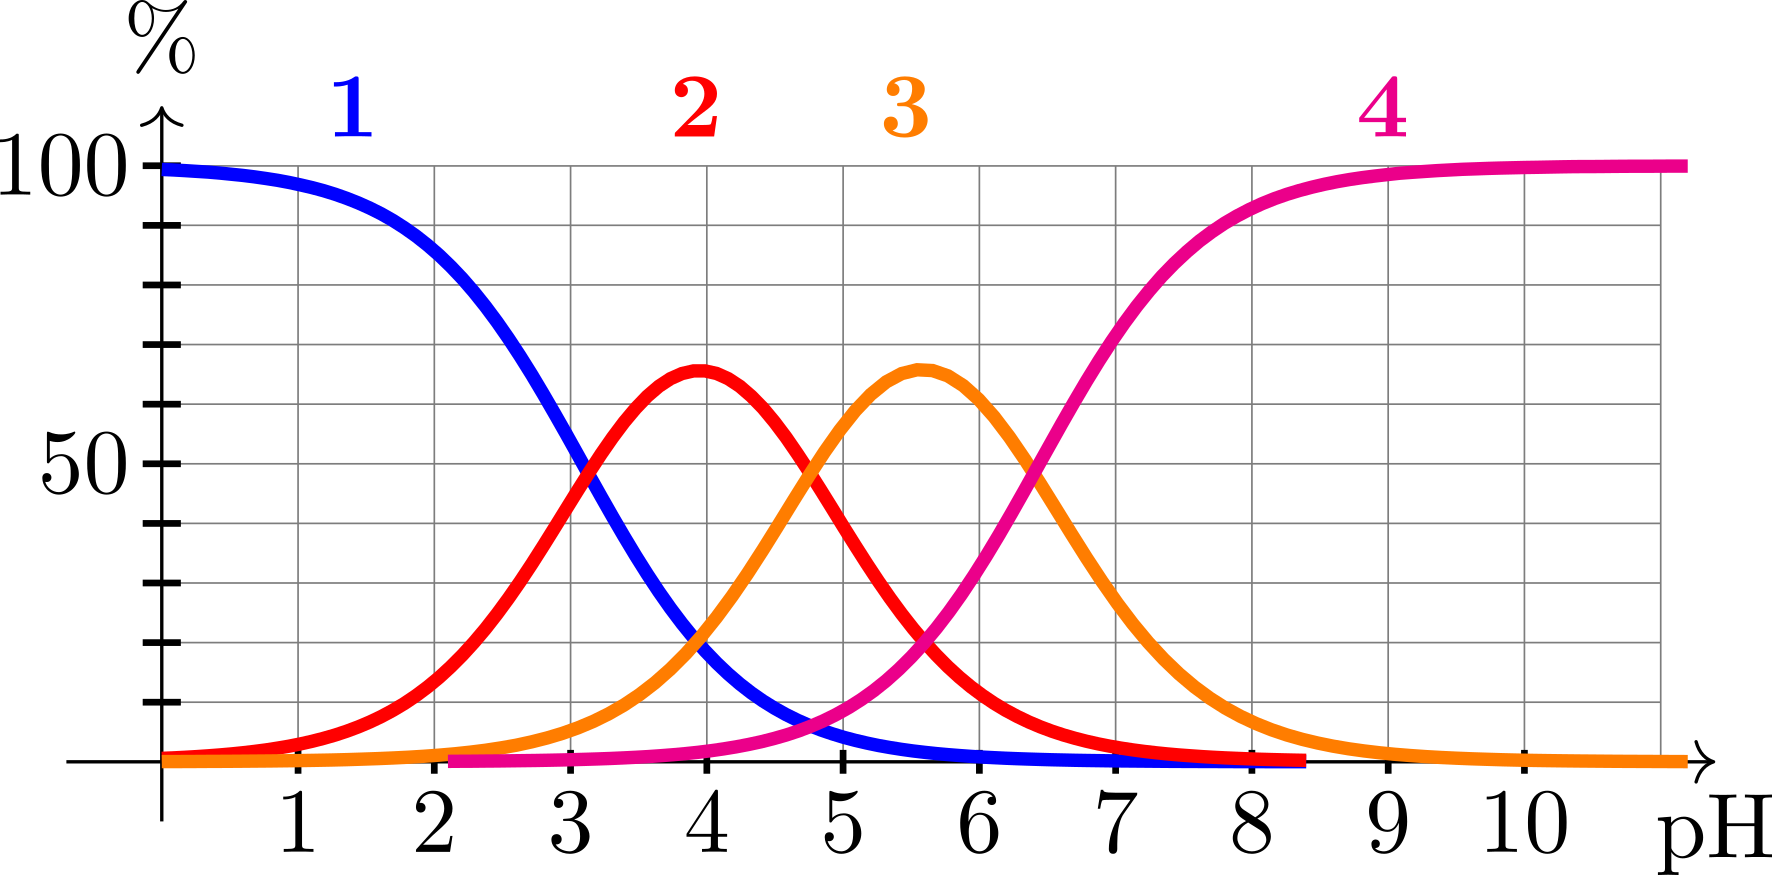
\includegraphics[width=\linewidth]{citrique}
		\end{center}
	\end{minipage}
}
\QR{%
	Associer à chaque courbe l'espèce correspondante.
}{%
	\begin{center}
		\includegraphics[width=.5\linewidth]{distrib_ex2}
	\end{center}
}
\QR{%
	Déterminer par lecture graphique les $\pk$ des trois premières acidités.
}{%
	\[
		\pk[A,1] \approx 3
		\quad ; \quad
		\pk[A,2] \approx \num{4.8}
		\quad ; \quad
		\pk[A,3] \approx \num{6.4}
	\]
}
\QR{%
	Le pH mesuré d'un jus de citron est de \num{2.5}. Donner sa composition en
	terme de pourcentage de chaque espèce.
}{%
	\[
		\alpha(\ce{H_4Cit}) \approx 69\%
		\quad ; \quad
		\alpha(\ce{H_3Cit^-}) \approx 29\%
		\quad ; \quad
		\alpha(\ce{H_2Cit^2-}) \approx 2\%
	\]
}

\resetQ
\section{État d'équilibre d'une base faible}
L'ion phosphate \ce{PO4^3-} est une base faible, qui intervient dans les couples
\ce{HPO4^2-}/\ce{PO4^3-} de $\pk = \num{12.3}$. On l'introduit en solution
aqueuse à la concentration initiale $c_0 = \SI{1e-1}{mol.L^{-1}}$.
\QR{%
	Déterminer la composition du système à l'équilibre, ainsi que le pH.
}{%
	\noindent
	\begin{minipage}[c]{.30\linewidth}
		\vspace{0pt}
		\begin{center}
			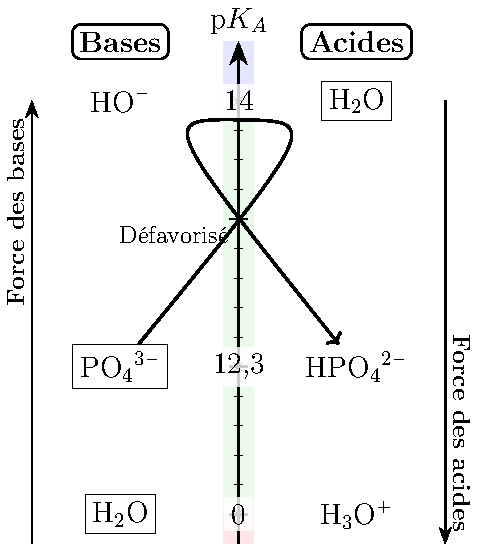
\includegraphics[width=\linewidth]{gamma_ex3}
			\captionof{figure}{Échelle $\pk$}
		\end{center}
	\end{minipage}
	\hfill
	\begin{minipage}[c]{.69\linewidth}
		Pour trouver la réaction en jeu, on trace l'échelle de $\pk$. La réaction
		prépondérante est celle entre la base la plus forte, \ce{PO4^3-}, et l'acide
		le plus fort, ici l'eau. Ainsi~:
		\begin{center}
			\def\rhgt{0.35}
			\centering
			\begin{tabularx}{\linewidth}{|l|c||YdYdYdY|}
				\hline
				\multicolumn{2}{|c||}{
					$\xmathstrut{\rhgt}$
				\textbf{Équation}}    &
				$\ce{PO_4^3-\aqu{}}$  & $+$              &
				$\ce{H_2O\liq{}}$     & $\ra$            &
				$\ce{HPO_4^2-\aqu{}}$ & $+$              &
				$\ce{HO^-\aqu}$                            \\
				\hline
				$\xmathstrut{\rhgt}$
				Initial               & $x = 0$          &
				$c_0$                 & \vline           &
				excès                 & \vline           &
				$0$                   & \vline           &
				$0$                                        \\
				\hline
				$\xmathstrut{\rhgt}$
				Final                 & $x_f = x_{\equ}$ &
				$c_0 - x_{\equ}$      & \vline           &
				excès                 & \vline           &
				$x_{\equ}$            & \vline           &
				$x_{\equ}$                                 \\
				\hline
			\end{tabularx}
		\end{center}
		Réaction défavorisée ($\gamma$) $\Ra K^\circ = 10^{\pk[a]-\pk[e]} =
			10^{\num{-1.7}}$~; or
		\begin{gather*}
			K = \frac{x\ind{eq}^2}{c_0 - x\ind{eq}}
			\Lra
			x\ind{eq}^2 + K x\ind{eq} - K c_0 = 0
		\end{gather*}
	\end{minipage}
	\vspace{-15pt}
	\begin{gather*}
		\\\Ra
		\Delta = K^2 + 4Kc_0
		\qet
		x_{\equ,\pm} = - \frac{K \pm \sqrt{K^2+4Kc_0}}{2}
		\Ra
		\left\{
		\begin{array}{ll}
			x_{\equ,-} & = \SI{-5.6e-2}{mol.L^{-1}}
			\\
			x_{\equ,+} & = \SI{3.2e-2}{mol.L^{-1}}
		\end{array}
		\right.
	\end{gather*}
	La réaction étant en sens direct forcément (pas de réactifs au début), on
	prend la solution positive, et ainsi
	\begin{gather*}
		\xul{x\ind{eq} = \SI{3.2e-2}{mol.L^{-1}}}
		\\
		\beforetext{Soit}
		[\ce{PO_4^2-}]\ind{eq} = \SI{6.3e-2}{mol.L^{-1}}
		\quad ; \quad
		[\ce{HPO_4^2-}]\ind{eq} = \SI{3.2e-2}{mol.L^{-1}} = [\ce{HO-}]\ind{eq}
		\Lra \pH = \num{12.8}
	\end{gather*}
}

\resetQ
\section{Iodure de plomb}
\begin{blocQR}
	\item Une solution contient initialement des ions \ce{Pb^2+} à la concentration
	$c = \SI{1e-1}{mol.L^{-1}}$, et des ions iodure \ce{I-} de même
	concentration. On donne $\pk[s](\ce{PbI_2}) = 8$.
	\QR{%
		Déterminer les concentrations en ions \ce{Pb^2+} et \ce{I-} dans l'état
		final.
	}{%
		\begin{center}
			\def\rhgt{0.35}
			\centering
			\begin{tabularx}{\linewidth}{|l|c||YdYdY|}
				\hline
				\multicolumn{2}{|c||}{
					$\xmathstrut{\rhgt}$
				\textbf{Équation}}   &
				$\ce{Pb^{2+}\aqu}$   & $+$                    &
				$2\ce{I^-\aqu}$      & $=$                    &
				$\ce{PbI_2\sol}$                                \\
				\hline
				$\xmathstrut{\rhgt}$
				Initial              & $\xi = 0$              &
				$cV$                 & \vline                 &
				$cV$                 & \vline                 &
				$0$                                             \\
				\hline
				$\xmathstrut{\rhgt}$
				Final                & $\xi_f = \xi\ind{max}$ &
				$cV - \xi\ind{max}$  & \vline                 &
				$cV - 2\xi\ind{max}$ & \vline                 &
				$\xi\ind{max}$                                  \\
				\hline
			\end{tabularx}
		\end{center}
		\begin{gather*}
			K^\circ = \frac{1}{K_s} = \num{e8}
			\qet
			Q_{r,i} = \frac{{c^\circ}^3}{c^3} = \num{e3} \ll \num{e8}
		\end{gather*}
		La réaction se fait donc dans le \textbf{sens direct} et est
		\textbf{totale}. On suppose donc que l'état final est
		$\xi\ind{eq}=\xi\ind{max}$, et on cherche $\xi\ind{max}$~:
		\begin{gather*}
			\left\{
			\begin{array}{ll}
				cV - \xi\ind{max}  & =0
				\\
				cV - 2\xi\ind{max} & =0
			\end{array}
			\right.
			\Lra
			\left\{
			\begin{array}{ll}
				\xi\ind{max} & = cV \tikzmark{MOU}
				\\
				\xi\ind{max} & \frac{cV}{2}
			\end{array}
			\right.
			\Ra
			\boxed{\xi\ind{max} = \frac{cV}{2}}
			\\\beforetext{Ainsi}
			\boxed{
				n_{\ce{PbI_2},\equ} = \frac{cV}{2}
				\quad ; \quad
				[\ce{I=}]\ind{eq} = \ep
				\quad ; \quad
				[\ce{Pb^2+}]\ind{eq} = \frac{c}{2}
			}
		\end{gather*}
		\begin{tcb}(impo){Important}
			On vérifie l'hypothèse de totalité en
			calculant $\ep$~:
			\[
				K = \frac{{c^\circ}^2}{\ep \frac{c}{2}}
				\Lra
				\ep = \frac{2}{Kc} = \SI{2e-7}{mol.^{-1}} \ll  \frac{c}{2}
			\]
			C'est bien vérifié \faIcon{check}~!
		\end{tcb}
	}
	\QR{%
		Même question si $c = \SI{2e-5}{mol.L^{-1}}$
	}{%
		\begin{gather*}
			c = \SI{2e-5}{mol.L^{-1}}
			\quad \Ra \quad
			Q_{r,i} = \num{1.25e14} > K^\circ
		\end{gather*}
		On devrait donc aller dans le sens indirect, ce qui n'est pas possible~: le
		système n'évolue pas.
	}
	\item
	\QR{%
		Déterminer la solubilité de l'iodure de plomb dans de l'eau pure.
	}{%
		\begin{enumerate}[label=\sqenumi]
			\item ~
			      \vspace{-18pt}
			      \begin{center}
				      \def\rhgt{0.35}
				      \centering
				      \begin{tabularx}{\linewidth}{|l|c||YdYdY|}
					      \hline
					      \multicolumn{2}{|c||}{
						      $\xmathstrut{\rhgt}$
					      \textbf{Équation}} &
					      $\ce{PbI_2\sol}$   & $=$                  &
					      $\ce{Pb^{2+}\aqu}$ & $+$                  &
					      $2\ce{I^-\aqu}$                             \\
					      \hline
					      $\xmathstrut{\rhgt}$
					      Initial            & $\xi = 0$            &
					      $n$                & \vline               &
					      $0$                & \vline               &
					      $0$                                         \\
					      \hline
					      $\xmathstrut{\rhgt}$
					      Final              & $\xi_f = \xi_{\equ}$ &
					      $n - \xi_{\equ}$   & \vline               &
					      $\xi_{\equ}$       & \vline               &
					      $2\xi_{\equ}$                               \\
					      \hline
				      \end{tabularx}
			      \end{center}
			\item \leavevmode\vspace*{-27pt}\relax
			      \begin{gather*}
				      \beforetext{Par définition,}
				      n\ind{dis,max} = \xi\ind{eq} = sV
				      \quad \Ra \quad
				      \left\{
				      \begin{array}{rl}
					      [\ce{Pb^2+}]\ind{eq} & = s
					      \\{}
					      [\ce{I-}]\ind{eq}    & = 2s
				      \end{array}
				      \right.
			      \end{gather*}
			\item \leavevmode\vspace*{-30pt}\relax
			      \begin{gather*}
				      \beforetext{Or,}
				      K_s =
				      \frac{[\ce{Pb^2+}]\ind{eq}\times[\ce{I-}]^2\ind{eq}}{{c^\circ}^3} =
				      4\left( \frac{s}{c^\circ} \right)^3
				      \\\Ra
				      \boxed{s = c^\circ \left( \frac{10^{-\pk[s]}}{4} \right)^{1/3}}
				      \quad \Ra \quad
				      \xul{s = \SI{2.0e-3}{mol.L^{-1}} = \SI{0.92}{g.mol^{-1}}}
			      \end{gather*}
		\end{enumerate}
	}
	\QR{%
		Même question dans une solution d'iodure de sodium $(\ce{Na+},\ce{I-})$ de
		concentration $c = \SI{1e-2}{mol.L^{-1}}$.
	}{%
		\begin{enumerate}[label=\sqenumi]
			\item ~
			      \vspace{-18pt}
			      \begin{center}
				      \def\rhgt{0.35}
				      \centering
				      \begin{tabularx}{\linewidth}{|l|c||YdYdY|}
					      \hline
					      \multicolumn{2}{|c||}{
						      $\xmathstrut{\rhgt}$
					      \textbf{Équation}} &
					      $\ce{PbI_2\sol}$   & $=$                  &
					      $\ce{Pb^{2+}\aqu}$ & $+$                  &
					      $2\ce{I^-\aqu}$                             \\
					      \hline
					      $\xmathstrut{\rhgt}$
					      Initial            & $\xi = 0$            &
					      $n$                & \vline               &
					      $0$                & \vline               &
					      $cV$                                        \\
					      \hline
					      $\xmathstrut{\rhgt}$
					      Final              & $\xi_f = \xi_{\equ}$ &
					      $n - \xi_{\equ}$   & \vline               &
					      $\xi_{\equ}$       & \vline               &
					      $cV + 2\xi_{\equ}$                          \\
					      \hline
				      \end{tabularx}
			      \end{center}
			\item \leavevmode\vspace*{-27pt}\relax
			      \begin{gather*}
				      \beforetext{Par définition,}
				      n\ind{dis,max} = \xi\ind{eq} = sV
				      \quad \Ra \quad
				      \left\{
				      \begin{array}{rl}
					      [\ce{Pb^2+}]\ind{eq} & = s
					      \\{}
					      [\ce{I-}]\ind{eq}    & = c + 2s
				      \end{array}
				      \right.
			      \end{gather*}
			\item \leavevmode\vspace*{-25pt}\relax
			      \begin{gather*}
				      \beforetext{Or,}
				      {c^\circ}^3K_s =
				      s \left( c+2s \right)^2 =
				      s c^2 + 4cs^2 + 4s^3
			      \end{gather*}
			      La résolution d'équation d'ordre 3 n'est pas au programme. On
			      doit trouver une astuce nous permettant de négliger quelque
			      chose. Ici, on peut supposer que $s \ll c$~: en effet, dans le
			      meilleur des cas avec le calcul précédent on a $s =
				      \SI{1.2e-3}{mol.L^{-1}}$ et l'effet d'ion commun ne fait que
			      baisser la solubilité, pas l'augmenter. Comme $c =
				      \SI{1e-2}{mol.L^{-1}}$, cette hypothèse est plausible.
			      \smallbreak
			      Dans ce cas, $c+2s \approx c$, et ainsi
			      \[
				      K_s = sc^2
				      \Lra
				      \boxed{s = \frac{K_s}{c^2}}
				      \Ra
				      \xul{s = \SI{1.0e-4}{mol.L^{-1}}}
			      \]
			      Ce qui vérifie par la même occasion l'hypothèse.
		\end{enumerate}
	}
\end{blocQR}

\resetQ
\section{Domaine d'existence de l'hydroxyde de fer II}
\enonce{%
	On considère l'hydroxyde de fer II \ce{Fe(OH)_2} de $\pk[s] = \num{15}$.
}
\QR{%
	Quelle est la valeur de $\prm \ce{OH} = - \log \frac{[\ce{HO-}]}{c^\circ}$ de
	début de précipitation de \ce{Fe(OH)_2} à partir d'une solution en ions
	\ce{Fe^2+} à la concentration $c_0 = \SI{1e-2}{mol.L^{-1}}$~?
}{%
	On a
}
\QR{%
	En déduire le pH de début de précipitation.
}{%
	solu
}
\QR{%
	Indiquer sur un diagramme, avec le pH en abscisse, les domaines de
	prédominance des ions \ce{Fe^2+} et d'existence du solide.
}{%
	solu
}

\resetQ
\section{Stabilité de solutions}
\enonce{%
	On considère les couples acido-basiques suivants~:
	\[
		\pk[A,1]\left( \ce{HCOOH}/\ce{HCOO-} \right) = \num{3.7}
		\qquad
		\pk[A,2]\left(\ce{HClO}/\ce{ClO-}\right) = \num{7.5}
	\]
}
\QR{%
	Tracer un diagramme de prédominance contenant les domaines des 4 espèces à
	considérer.
}{%
	solu
}
\begin{blocQR}
	\item
	Déterminer les les deux mélanges suivants sont stables (aucune réaction
	quantitative n'a lieu)~:
	\QR{%
		$n_{\ce{HCOOH},0} = \SI{1}{mol}$ et $n_{\ce{HClO},0} = \SI{1}{mol}$ dans $V =
			\SI{1}{L}$
	}{%
		solu
	}
	\QR{%
		$n_{\ce{ClO-,0} = \SI{1}{mol}}$ et $n_{\ce{HCOOH},0} = \SI{1}{mol}$ dans $V =
			\SI{1}{L}$
	}{%
		solu
	}
\end{blocQR}

\resetQ
\section{Titrage de l'acide acétique d'un vinaigre}
\enonce{%
	Le vinaigre est obtenu par fermentation acétique, soit d'une solution aqueuse
	d'éthanol (vinaigre d'alcool), soit d'un vin (vinaigre de vin). La
	fermentation est effectuée par des bactéries, qui oxydent l'éthanol
	\ce{CH3CH2OH} en acide éthanoïque \ce{CH3CO2H}, aussi appelé acide acétique.
	\smallbreak
	La base conjuguée de l'acide éthanoïque est l'ion éthanoate \ce{CH3CO2^-}, de
	$\pk = \num{4.75}$. On étudie un vinaigre d'alcool du commerce, dont le pH
	vaut \num{2.6}. Afin de doser l'acidité de ce vinaigre, on prépare tout
	d'abord une solution aqueuse contenant \SI{10.0}{mL} du vinaigre dans
	\SI{200.0}{mL} d'eau.
	\smallbreak
	\noindent
	\begin{minipage}[c]{.55\linewidth}
		Un volume $V_1 = \SI{20.0}{mL}$ de cette solution diluée est placée dans un
		bécher, dans lequel on place deux électrodes pour la mesure du pH. De l'eau
		est ajoutée pour obtenir l'immersion dans les électrodes. Une solution
		aqueuse de soude \ce{NaOH} de concentration $c = \SI{0.10}{mol.L^{-1}}$ est
		placée dans une burette. Le dosage consiste à verser progressivement cette
		solution dans le bécher, tout en suivant l'évolution du pH. La figure
		ci-contre montre le pH en fonction du volume $V$ de solution de \ce{NaOH}
		versé.
    \smallbreak
	L'équivalence est repérée par le saut de pH, qui se produit pour un volume
	versé $V\ind{eq} = \SI{12.75}{mL}$ (volume pour lequel la dérivée du pH en
	fonction de $V$ est maximale).
	\end{minipage}
	\hfill
	\begin{minipage}[c]{.45\linewidth}
		\vspace{0pt}
		\begin{center}
			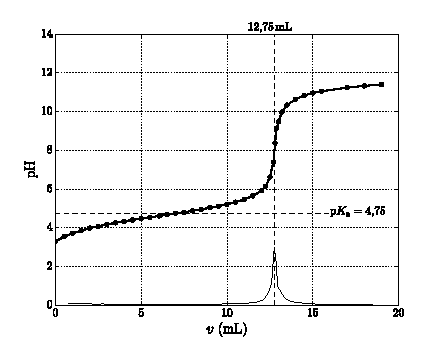
\includegraphics[width=\linewidth]{titrage_vinaigre}
		\end{center}
	\end{minipage}
}
\QR{%
	Faire des schémas des différentes étapes en notant les quantités et
	concentrations importantes.
}{%
	solu
}
\QR{%
	Écrire la réaction de \ce{CH3CO2H} avec \ce{HO-}. Calculer sa constante
	d'équilibre et commenter.
}{%
	solu
}
\QR{%
	Calculer le nombre de moles d'acide éthanoïque dans la solution diluée dosée,
	puis la concentration en acide éthanoïque dans le vinaigre non dilué.
}{%
	solu
}
\QR{%
	Calculer la masse d'acide éthanoïque pour \SI{100}{g} de vinaigre. On donne
	les masses molaires :
	\[
		M_{\ce{C}} = \SI{12.0}{g.mol^{-1}}
		\qquad
		M_{\ce{O}} = \SI{16.0}{g.mol^{-1}}
		\qquad
		M_{\ce{H}} = \SI{1.0}{g.mol^{-1}}
	\]
}{%
	solu
}
\QR{%
	Calculer les concentrations de \ce{CH3CO2H} et de \ce{CH3CO2^-} dans le
	vinaigre.
}{%
	solu
}

\resetQ
\section{Hydroxyde d'étain}
La solubilité $s$ de l'hydroxyde d'étain $\ce{Sn(OH)_2\sol{}}$ varie avec le pH
en raison des équilibres suivants~:
\begin{alignat}{3}
	\beforetext{$K_s=10^{\num{-25.2}}$}
	\ce{Sn^2+\aqu{}    & + 2 HO^-\aqu{} &  & = Sn(OH)_2\sol{}   & }
	\tag{S}\label{eq:RS}
	\\
	\beforetext{$K_{A,1}=10^{\num{-2.1}}$}
	\ce{Sn^2+\aqu{}    & + H_2O\liq{}   &  & = Sn(OH)^+\aqu{}   & + H+\aqu}
		\tag{1}\label{eq:R1}
	\\
		\beforetext{$K_{A,2}=10^{\num{-5.0}}$}
	\ce{Sn(OH)^+\aqu{} & + H_2O\liq{}   &  & = Sn(OH)_2\aqu{}   & + H+\aqu}
	\tag{2}\label{eq:R2}
	\\
	\beforetext{$K_{A,3}=10^{\num{-9.5}}$}
	\ce{Sn(OH)_2\aqu{} & + H_2O\liq{}   &  & = Sn(OH)_3^-\aqu{} & + H+\aqu}
	\tag{3}\label{eq:R3}
\end{alignat}
On donne le graphe $\log s = f(\pH)$ ci-dessous~:
\begin{figure}[htbp!]
	\centering
	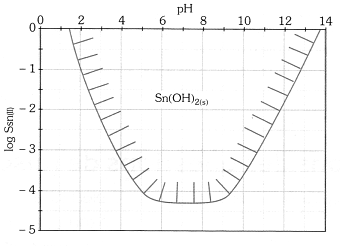
\includegraphics[width=.5\linewidth]{snoh2-white}
	\label{fig:snoh2}
\end{figure}
\QR{%
	Indiquer sur une échelle de pH les domaines de prédominance des différentes
	formes solubles de l'étain considérées ici.
}{%
	solu
}
\QR{%
	Déterminer la solubilité de l'étain en ne considérant que l'équilibre~:
	\begin{gather*}
		\beforetext{$K^\circ$}
		\ce{Sn(OH)_2\aqu{} = Sn(OH)_2\sol{}}
	\end{gather*}
}{%
	solu
}
\QR{%
	Exprimer la solubilité $s$ de l'hydroxyde d'étain pour tout pH, en considérant
	cette fois tous les équilibres. Retrouver alors la pente de la courbe pour
	$\pH > \num{10.5}$.
}{%
	solu
}

\resetQ
\section{Diacide fort}
\enonce{%
	On considère une solution d'acide sulfurique \ce{H2SO4} de concentration $c_0
		= \SI{0.010}{mol.L^{-1}}$.
}
\QR{%
	En considérant que l'acide sulfurique est un diacide fort, calculer le pH de
	la solution.
}{%
	solu
}
\QR{%
	En réalité, la première acidité de l'acide sulfurique est forte, et la seconde
	a un $\pk (\ce{HSO_4^-}/\ce{SO_4^2-}) = \num{1.9}$. Déterminer le pH en tenant
	compte de cette modification.
}{%
	solu
}

\resetQ
\section{Solubilités dans l'eau pure de différents précipités}
\enonce{%
	Déterminer la solubilité dans l'eau pure $s$ de chacun des composés
	ci-dessous, en supposant que les ions formés lors de la dissociation des
	solides ne réagissent pas avec l'eau et que l'ion \ce{Zn^2+} apparaît dans
	chaque dissolution.
}
\QR{%
	$\ce{ZnCO3\sol{}}$ de $\pk[s,1] = \num{10.8}$.
}{%
	solu
}
\QR{%
	$\ce{ZnCN_2\sol{}}$ de $\pk[s,2] = \num{12.6}$.
}{%
	solu
}
\QR{%
	$\ce{Zn_3(PO_4)_2\sol{}}$ de $\pk[s,3] = \num{32.0}$.
}{%
	solu
}

\resetQ
\section{Mesure de la constante d'acidité d'un indicateur coloré.}
\enonce{%
	À partir du spectre d'absorption de la forme acide notée \ce{HIn} du bleu de
	bromothymol (BBT), on détermine la longueur d'onde correspondant à son maximum
	d'absorption $\lambda_1 = \SI{430}{nm}$. On détermine de même la longueur
	d'onde du maximum d'absorption de la forme basique \ce{In-} $\lambda_2 =
		\SI{620}{nm}$.
}
\QR{%
	Quelle est la couleur d'une solution contenant uniquement \ce{HIn}~?
	uniquement \ce{In-}~?
}{%
	solu
}
\QR{%
	Quelle est la couleur d'une solution de BBT dans sa zone de virage~?
}{%
	solu
}
\QR{%
	Rappeler la loi de \textsc{Beer-Lambert} en précisant la signification des
	différents termes. Quelles sont les conditions de validité de cette loi~?
}{%
	solu
}
\enonce{%
	On mesure l'absorbance pour la longueur d'onde $\lambda_1$ de trois solutions
	contenant du BBT à une même concentration totale $c$~:
	\begin{itemize}
		\item En milieu fortement acide, on mesure $A_1 = \num{0.196}$~;
		\item En milieu fortement basique, on mesure $A_2 = \num{0.076}$~;
		\item Pour une solution $S$ à $\pH = \num{7.1}$, on mesure $A_S =
			      \num{0.140}$.
	\end{itemize}
}
\QR{%
	Montrer que le rapport des concentrations en forme acide et basique dans la
	solution $S$ peut s'écrire
	\[
		\frac{[\ce{HIn}]_S}{[\ce{In-}]_S} = \frac{A_1-A_S}{A_S-A_2}
	\]
}{%
	solu
}
\QR{%
	En déduire la valeur de $\pk(\ce{HIn}/\ce{In-})$.
}{%
	solu
}

\resetQ
\section{Titrage d'une amine}
\noindent
\begin{minipage}[c]{.55\linewidth}
	On veut déterminer par titrage la formule brute d'une amine
	\ce{C_nH_{2n+1}NH2}. Pour cela, on dissout une masse $m = \SI{0.146}{g}$ dans
	\SI{100}{mL} d'eau et on dose la solution obtenue par une solution d'acide
	chlorhydrique $(\ce{H+},\ce{Cl-})$ de concentration molaire $c_A =
		\SI{0.25}{mol.L^{-1}}$. On donne ci-contre la courbe de titrage $\pH = f(V)$,
	à laquelle sont superposées en traits fins deux courbes représentant les
	pourcentages respectifs des espèces \ce{C_nH_{2n+1}NH2} et
	\ce{C_nH_{2n+1}NH3+} en solution en fonction du volume $V$ de solution
	titrante versée.
	\smallbreak
\end{minipage}
\hfill
\begin{minipage}[c]{.45\linewidth}
	\vspace{0pt}
	\begin{center}
		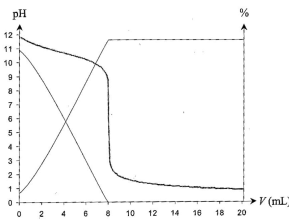
\includegraphics[width=\linewidth]{amine}
	\end{center}
\end{minipage}
\begin{tcb}(data)<lftt>{Données}
	\begin{itemize}
		\item $M_{\ce{H}} = \SI{1.0}{g.mol^{-1}}$~; $M_{\ce{C}} =
			      \SI{12.0}{g.mol^{-1}}$~; $M_{\ce{N}} = \SI{14.0}{g.mol^{-1}}$~;
		\item Zones de virage d'indicateurs colorés~:
		      \begin{itemize}
			      \item Phénolphtaléine \numrange{8.2}{10.0}
			      \item BBT \numrange{6.0}{7.6}
			      \item Vert malachite \numrange{0.2}{1.8}
		      \end{itemize}
	\end{itemize}
\end{tcb}

\QR{%
Attribuer les courbes de pourcentages aux deux espèces \ce{C_nH_{2n+1}NH2} et
\ce{C_nH_{2n+1}NH3+} et déterminer le $\pk$ du couple.
}{%
solu
}
\QR{%
	Écrire l'équation de la réaction. Calculer sa constante d'équilibre et
	justifier qu'elle peut servir de support de titrage.
}{%
	solu
}
\QR{%
	Justifier qualitativement l'allure de la courbe de pH, et en particulier
	l'existence du saut.
}{%
	solu
}
\QR{%
	Proposer un indicateur coloré adapté au repérage de l'équivalence.
}{%
	solu
}
\QR{%
	Déterminer la formule de l'amine.
}{%
	solu
}

\end{document}
